
\section{ Extracting thermal impedances using FEA simulations}


\subsection{Setup of the FEA Simulation to extract thermal impedances}

Representative power numbers are used to power each component. In each simulation run, all instances
of one type of component (e.g. the ABCs) are powered on in all six modules, keeping the rest off.
Average temperatures are measured for the following components (see below): HCC, ABC, FEAST, sensor.

\def\thcc{\ensuremath{\overline{T}_\text{nHCC}}}
\def\tabc{\ensuremath{\overline{T}_\text{nABC}}}
\def\tfeast{\ensuremath{\overline{T}_\text{FEAST}}}
\def\tsensor{\ensuremath{T_\text{sensor}}}
\def\Rm{\ensuremath{{\text{R}m}}}

\begin{itemize}
\item FEAST: a $3\times3$~mm $\times~350~\mu$m chip inside the shield box.
  \begin{itemize}
  \item The FEAST has an additional power term due to regulators for the AMAC -- see below.
  \end{itemize}
\item AMAC: a $3\times3$~mm $\times~350~\mu$m chip, roughly in the center of the power board
  \begin{itemize}
    \item The AMAC is powered using regulators located in the FEAST chip, with a power dissipation
      of the regulators corresponding to the voltage drop in the regulator (0.415~W) -- see Eq.~\ref{eq:amac_regulator}.
  \end{itemize}
\item HVMUX: Ignore for now
\item EOS (\highlight{3.20~W total, including both sides -- see Table~\ref{tab:power_numbers}.}) % (\highlight{3.03~W total, for both sides}):
  \begin{itemize}
  \item \highlight{Placement of these EOS power sources: ???}
%%     \item 1 lpGBT per side (\highlight{0.750~W $\times$ 2 sides})
%%     \item ``Rest'' (1 VTRX optical link per side?) (\highlight{.185~W $\times$ 2 sides}) ???
%%     \item FEAST on a single side (\highlight{1.12~W})
%%     \item DCDC2 converter on a single side (\highlight{0.21~W})
  \end{itemize}
\item Cooling: Constant 8000~W/m$^{2}$K, $-30$~C, no convection
\end{itemize}




\subsection{FEA Simulation Runs to extract thermal impedances}

For the extraction of the thermal impedances, a simplified set of input power parameters are used,
summarized in Table~\ref{tab:simulation_runs}.
In the FEA, the power is distributed over all 6 surfaces (\highlight{different from barrel treatment}).

\let\arraystretcha\arraystretch
\renewcommand\arraystretch{1.4} % 1.6
\begin{table}[h!]
\footnotesize
\begin{center}
\adjustbox{max width=\textwidth}{ %% just before tabular
\begin{tabular}{|l|l|l|l|} \hline
Simulation \# & Description                        & Input parameters           \\ \hline
1             & All HCCs powered on, rest off      & $P_\text{HCC}=0.413$~W     \\
2             & All ABCs powered on, rest off      & $P_\text{ABC}=0.149$~W     \\
3             & All FEASTs powered on, rest off    & $P_\text{FEAST}=1.5$~W$^*$ \\
%% \hline
%% \multicolumn{3}{|c|}{Extended simulations} \\ \hline
%% 4             & Tape ``powered'' on, rest off      & skip for now \\
%% 5             & HVMUX powered on, rest off         & skip for now \\
%% 6             & R$_\text{HV}$ powered on, rest off & skip for now \\
%% 7             & EOS                                & skip for now \\ % $P_\text{EOS}=3.03$~W$^{**}$
\hline \end{tabular}
} %% resizebox after tabular
\end{center}
\caption{ Description of the 3 thermal simulations required to obtain the thermal impedances.
}
\label{tab:simulation_runs}
\end{table}
\let\arraystretch\arraystretcha

$^*$ The actual nominal power of the FEAST varies for each module; however, for the simulation to extract
the thermal impedances, the power is set to 1.5~W for all FEASTs in the petal.\\






\subsection{Measurements performed in each run}

%% For each component, the temperature measured is the average of the top surface nodes of all
%% components of a given type, in a given module.

The average, min and max temperatures are taken over the volume of the elements (\highlight{different from barrel treatment}).
There are 45 measurements per simulation run in total.

The average temperatures can be measured either \highlight{on one side of the petal, or as the average of components on both sides 
of the petal}.

\begin{itemize}
\item $(\thcc)_\Rm$: The average HCC temperature of the $n$ HCCs in the module, for each module R$m$ (R0, R1, ... R5) (6~total)
\item $(\tabc)_\Rm$: The average ABC temperature of the $n$ ABCs in the module, for each module R$m$ (6~total)
\item $(\tfeast)_\Rm$: The temperature of the FEAST in the module, for each module R$n$ (6~total)
\item \tsensor, taken for R0, R1, R2, R3\_left, R3\_right, R4\_left, R4\_right, R5\_left, R5\_right (9~total) (27~total measurements):
\begin{itemize}
  \item $\tsensor^\text{Avg}$: The average sensor temperature taken over the volume of the sensor
  \item $\tsensor^\text{Max}$: The maximum sensor temperature in the module, for each module
  \item $\tsensor^\text{Min}$: The minimum sensor temperature in the module, for each module
\end{itemize}
\end{itemize}




\section{The Linear Model}

%% \subsection{Additional parameters in the linear model}
\subsection{Other assumed quantities}

Assumed quantities are below:
\begin{itemize}
\item $R_\text{EOS}=15.0$~K/W (guessed by Georg/Graham)
\item $R_\text{sensor}=0.02$~K/W (guessed by Georg/Graham)
\item $R_\text{tape}=0.01$~K/W per module (i.e. there are 6 such resistors in the petal, one
for each module). This is considered a worst-case value.
%% \item EOS DCDC2 efficiency: 0.88
%% \item $V_\text{hybrid}=1.5$~V
%% \item $I^\text{digital}_\text{HCC}=0.125$~A (before TID damage; TID-dependent)
%% \item $I^\text{analog}_\text{HCC}=0.075$~A
%% \item $I^\text{digital}_\text{ABC}=0.035$~A (before TID damage; TID-dependent)
%% \item $I^\text{analog}_\text{ABC}=0.066$~A
\end{itemize}

%% The AMAC:
%% \begin{itemize}
%% \item $V^{1.5V}_\text{AMAC} = 1.5$~V
%% \item $I^{1.5V}_\text{AMAC} = 0.045$~A
%% \item (Efficiency $\varepsilon^{1.5V}_\text{AMAC} = 0.65$\% -- not used in model)
%% \item $V^{3.0V}_\text{AMAC} = 3.0$~V
%% \item $I^{3.0V}_\text{AMAC}= 0.002$~A
%% \item (Efficiency $\varepsilon^{3.0V}_\text{AMAC} = 0.65$\% -- not used in model)
%% \end{itemize}

\begin{figure}[ht!]
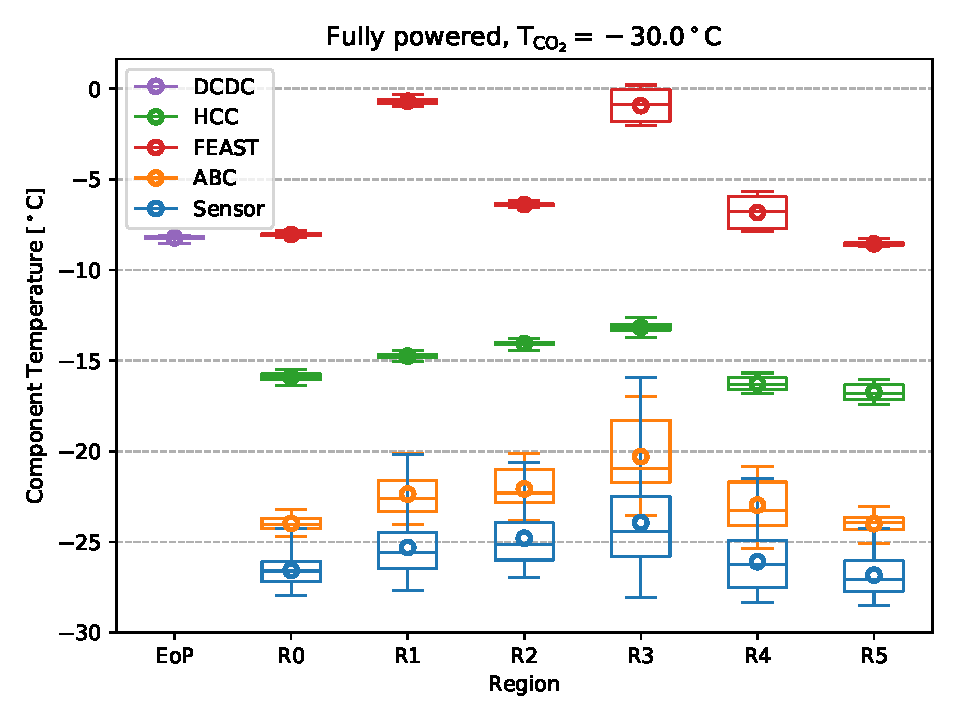
\includegraphics[width=0.49\linewidth]{figures/FEA_20171207_m30p0C_0p0Wm2C_DP1_ALL_S0.pdf}
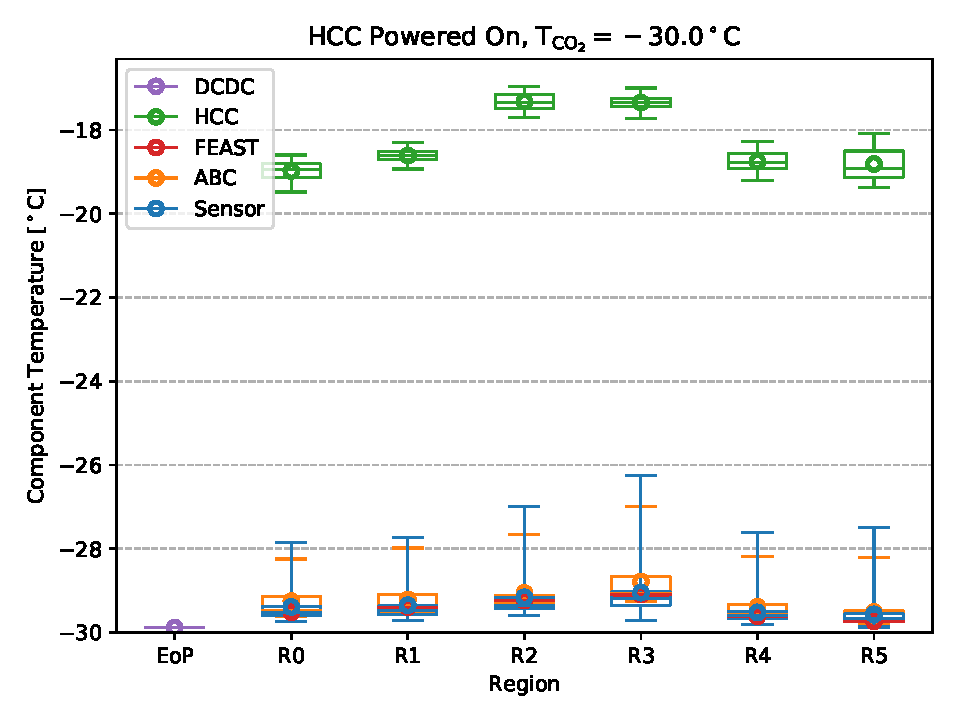
\includegraphics[width=0.49\linewidth]{figures/FEA_20171207_m30p0C_0p0Wm2C_DP1_ALL_S1.pdf}\\
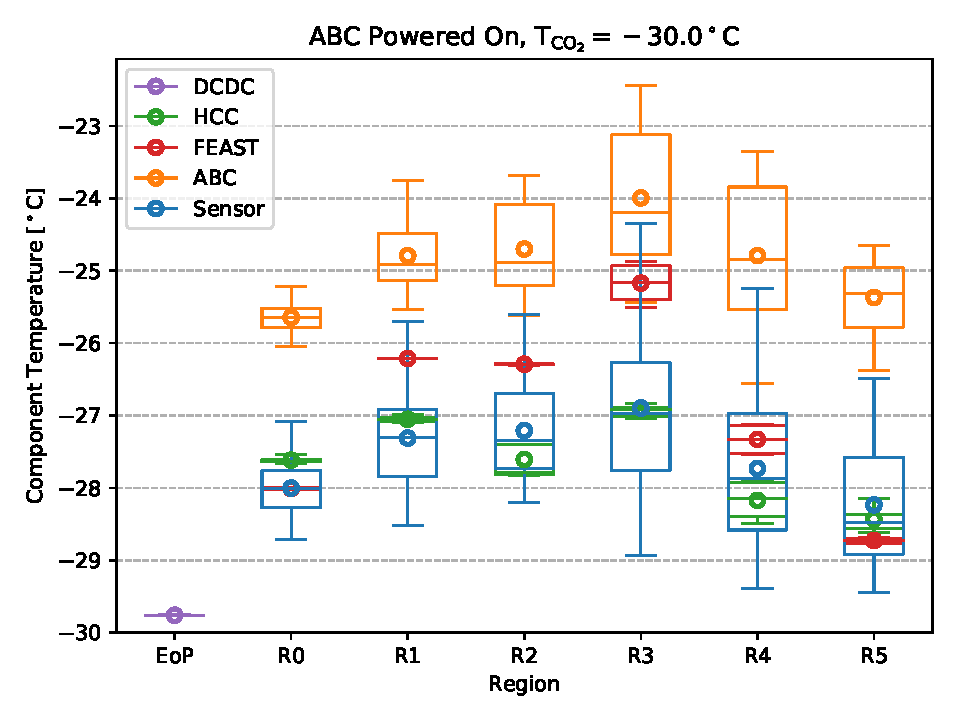
\includegraphics[width=0.49\linewidth]{figures/FEA_20171207_m30p0C_0p0Wm2C_DP1_ALL_S2.pdf}
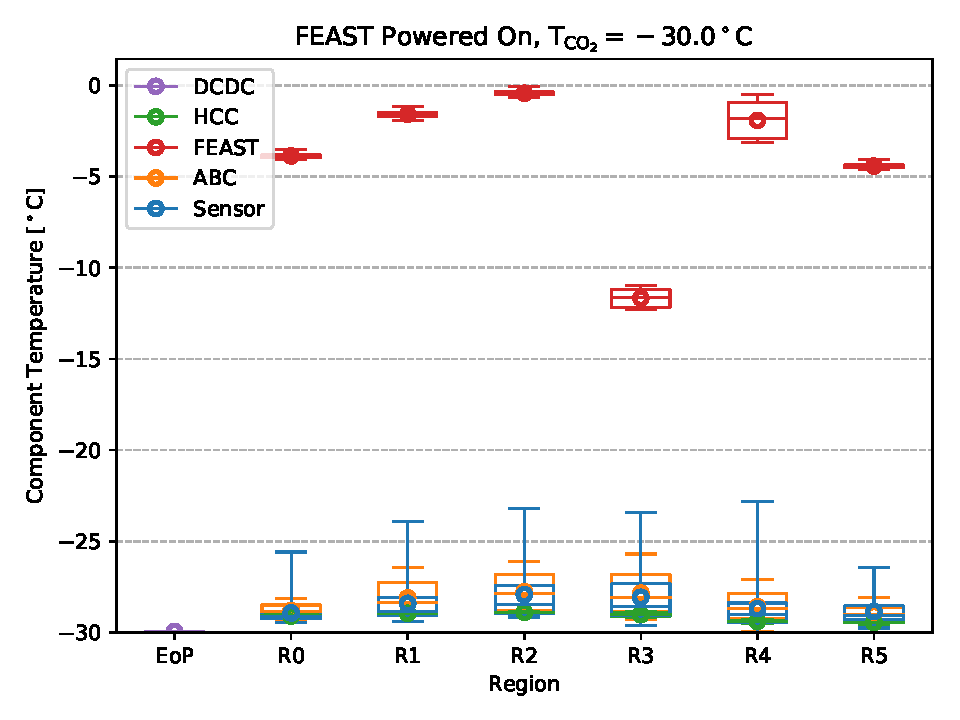
\includegraphics[width=0.49\linewidth]{figures/FEA_20171207_m30p0C_0p0Wm2C_DP1_ALL_S3.pdf}
\caption{Box-and-whisker plot of the four scenarios described in Table~\ref{tab:simulation_runs}.
The box is the interquartile range (middle 50\%) of the component's temperature, and the whiskers are
the minimum and maximum temperatures.}
\label{thermal_data}
\end{figure}

Table~\ref{tab:thermal_impedances} shows the thermal impedances calculated
from the FEA simulations.

%% \def\insulabc{$R_\text{ABC}\times n_\text{ABC}$\xspace}
%% \def\insulhcc{$R_\text{HCC}\times n_\text{HCC}$\xspace}
\def\insulabc{$(R\times n)_\text{ABC}$\xspace}
\def\insulhcc{$(R\times n)_\text{HCC}$\xspace}
\def\insulfeast{$(R\times n)_\text{FEAST}$\xspace}

%
\let\arraystretcha\arraystretch
\renewcommand\arraystretch{1.1} % 1.6
\begin{table}[h]
\begin{center}
\adjustbox{max width=\textwidth}{ %% just before tabular
\begin{tabular}{|l|cc|c|c|c|c|c|c|} \hline
       &             &              &  \multicolumn{2}{c|}{FEAST}     & \multicolumn{2}{c|}{ABC}   & \multicolumn{2}{c|}{HCC}   \\
Module & $R_C$ [K/W] & $R_M$ [K/W]  & $ R_\text{FEAST}$ & \insulfeast & $R_\text{ABC}$ & \insulabc & $R_\text{HCC}$ & \insulhcc \\ \hline
R0     & \multicolumn{2}{c|}{0.802} &            16.627 &      16.627 &          0.927 &    15.759 &         12.485 &    24.970 \\
R1     & \multicolumn{2}{c|}{0.991} &            17.936 &      17.936 &          0.661 &    13.881 &         12.719 &    25.438 \\
R2     & \multicolumn{2}{c|}{1.410} &            18.282 &      18.282 &          1.529 &    18.348 &         13.833 &    27.666 \\
R3     & \multicolumn{2}{c|}{0.873} &            11.361 &      22.722 &          0.582 &    16.296 &\phantom{0}6.808&    27.232 \\
R4     & \multicolumn{2}{c|}{0.744} &            17.847 &      17.847 &          1.316 &    21.056 &         12.669 &    25.338 \\
R5     &              0.486 & 0.690 &            16.470 &      16.470 &          1.151 &    20.718 &         12.905 &    25.810 \\ \hline
SS EOS    &           0.719 & 0.393      & \multicolumn{2}{c|}{19.650} &         1.003 &    20.060 &         12.305 &    24.610 \\
SS middle &   \multicolumn{2}{c|}{1.160} & \multicolumn{2}{c|}{19.752} &         0.928 &    18.560 &         13.157 &    26.314 \\
LS EOS    &           0.811 & 0.427      & \multicolumn{2}{c|}{19.602} &         2.194 &    21.940 &         24.195 &    24.195 \\
LS middle &   \multicolumn{2}{c|}{1.360} & \multicolumn{2}{c|}{19.663} &         2.141 &    21.410 &         25.174 &    25.174 \\
%% in [degC/W]  RC       RM       RS      REOS    RABC     RHCC      RFEAST
%% SS EOS       0.719    0.393    0.02    15.0    1.003    12.305    19.650
%% SS middle    1.160             0.02       -    0.928    13.157    19.752
%% LS EOS       0.811    0.427    0.02    15.0    2.194    24.195    19.602
%% LS middle    1.360             0.02       -    2.141    25.174    19.663
\hline \end{tabular}
} %% resizebox after tabular
\end{center}
\caption{Effective thermal impedances calculated from Yu-Heng's numbers (in K/W).
For instances where you have $n$ components, the thermal insulance (inverse of HTC) is also calucated, simply
in units of {${(\text{Area}_\text{1-device})\cdot\text{K/W}}$}.
}
\label{tab:thermal_impedances}
\end{table}
\let\arraystretch\arraystretcha
